%% ------------------------------------------------------------------------- %%
\chapter{Problema}
\label{cap:problema}

Conforme o capítulo~\ref{cap:trabalhos-relacionados}, há várias pesquisas sobre o problema de perguntas e respostas no processamento de linguagem natural. Porém, como observado pelo trabalho da \cite{yao-2018} e apontado na seção~\ref{sec:algumas_referencias}, não há muita pesquisa sobre o problema de pares de perguntas e códigos-fontes. A partir de 2014, o StackOverFlow passou a disponibilizar a base de dados livremente. Diversas pesquisas foram feitas utilizando esta base de dados. E uma frente explorada pela \cite{yao-2018} e outros pesquisadores, é tentar resolver o problema de pergunta e resposta utilizando os dados do \textit{StackOverFlow}.

%------------------------------------------------------
\section{Problema de pares de perguntas e códigos-fontes do \textit{StackOverFlow}}

O problema de pares de perguntas e códigos-fontes já foi discutido na seção~\ref{sec:algumas_referencias}. E um dos obstáculos mencionados, é a obtenção de dados para o treinamento de modelos supervisionados. Desde 2014, o site \textit{StackOverFlow} disponibiliza sua base de perguntas e respostas através do site \cite{sof-2019}. Estes dados também podem ser consultados através do site \textit{BigQuery} do \cite{bigquery-2019} também. Numa consulta rápida, até 20 de março de 2019, havia mais de 17 milhões de perguntas em diversos tópicos de programação. Dúvidas sobre Python e SQL totalizam juntas mais de 2 milhões e meio.

\begin{figure}[h]
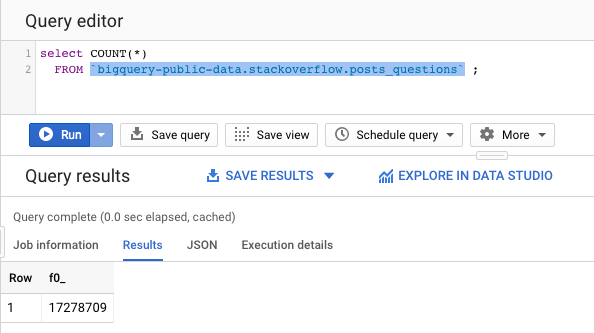
\includegraphics[width=12cm]{src/figuras/cap-problema/post-questions-total.png}
\caption{Total de perguntas no \textit{StackOverFlow}. Google and the Google logo are registered trademarks of Google LLC, used with permission.}
\label{fig:bigquery-total-questions-stackoverflow}
\end{figure}

\begin{figure}[h]
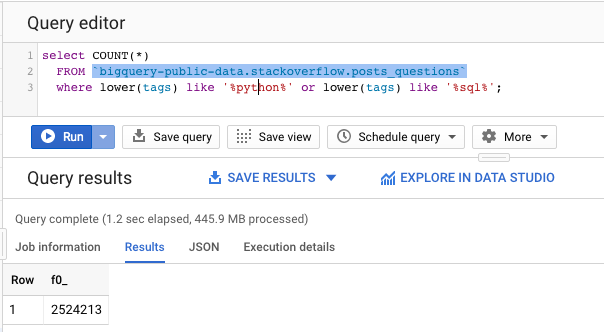
\includegraphics[width=12cm]{src/figuras/cap-problema/post-questions-python-sql-total.png}
\caption{Total de perguntas sobre Python e SQL no \textit{StackOverFlow}. Google and the Google logo are registered trademarks of Google LLC, used with permission.}
\label{fig:bigquery-total-questions-python-sql-stackoverflow}
\end{figure}

Somente com estes números, vê-se o potencial do \textit{StackOverFlow} como fonte de perguntas em linguagem natural e a sua solução em código fonte \cite{yao-2018}. Porém, ao utilizar o \textit{StackOverFlow} como fonte de repositório de pares de perguntas e códigos-fontes, é necessário levar em consideração quais assuntos é permitido fazer a pergunta. De acordo com o guia de boas práticas do \cite{stackoverflow-questions-topics-2019}, são permitidas perguntas sobre:

\begin{itemize}
    \item um problema específico de programação
    \item um algoritmo de programação
    \item ferramentas de programação
    \item problemas referentes a desenvolvimento de software
\end{itemize}



\subsection{Detalhes do dataset}

 - Tamanho do dataset inicial
 - Dados sobre as perguntas, respostas (tamanho, quantidade de palavras etc.)

%------------------------------------------------------
\section{Arquitetura proposta} 

- Uso da rede LSTM/CNN 
       - Utilizando cosine similarity
       - Uso do word2vec para pergunta (linguagem natural) e outro para código (linguagem estruturada) - Verificar também se é viável usar o artigo Deep contextualized word representations ELMo representation (ao invés de word2vec) (According to the article: "We show that
these representations can be easily added to
existing models and significantly improve the
state of the art across six challenging NLP
problems, including question answering, textual entailment and sentiment analysis." )





